\chapter{Marco Teórico}
\label{chap:marco_teorico}

\lettrine{E}{n} este capítulo se presenta una breve explicación de las técnicas implementadas en este trabajo.
Se describen los conceptos de planificación simbólica (\gls{htn}), aprendizaje por imitación (\gls{il}) y aprendizaje por refuerzo (\gls{rl}),
así como las familias de algoritmos en las que se basan.

\section{Planificación Simbólica}
La planificación simbólica se caracteriza por ser un enfoque interpretable debido a su funcionamiento basado en reglas,
las cuales definen los estados, acciones y objetivos sobre los que opera el agente, determinando el mundo sobre el que actúa y el plan que debe seguir para cumplir su objetivo.
Dentro de la planificación simbólica existen diferentes paradigmas:

\begin{itemize}
    \item \gls{strips}~\cite{DBLP:journals/ai/FikesN71}: utiliza un \gls{solver} que, dado un mundo (estado), 
    un conjunto de operadores aplicables (acciones) que transforman el mundo y un objetivo a alcanzar, 
    encuentra una secuencia de acciones que transforma el estado inicial en uno que cumple el objetivo.

    \item \gls{sat}~\cite{DBLP:conf/ecai/KautzS92}: utiliza técnicas de satisfacibilidad para encontrar planes que 
    cumplan con las restricciones del dominio. Al igual que \gls{strips}, utiliza un \gls{solver}.

    \item \gls{htn}~\cite{DBLP:conf/aips/ErolHN94, DBLP:conf/ijcai/OntanonB15}: con una base similar a \gls{strips}, 
    pero de forma más jerárquica. En lugar de buscar la secuencia de acciones únicamente a partir del objetivo, 
    las tareas se descomponen recursivamente en subtareas y acciones, formando un árbol de descomposición.
\end{itemize}

El paradigma seleccionado para este trabajo es el de las \gls{htn}, por su capacidad para modelar comportamientos 
complejos de forma jerárquica, similar a la forma en la que se progresa en \textit{Minecraft}.
En lugar de partir únicamente de un objetivo y dejar que el \gls{solver} busque la secuencia de acciones, 
una \gls{htn} descompone el objetivo en tareas, para las cuales el programador indica cómo se resuelven o cómo 
se dividen en subtareas más sencillas.
La planificación se convierte entonces, en el recorrido de un árbol de tareas y subtareas.
El comportamiento del agente se basa en tareas, que pueden ser de tres tipos:

\begin{itemize}
    \item \textbf{Primitiva}: se resuelve ejecutando una única acción directa sobre el mundo, 
    siempre que se cumplan sus precondiciones.

    \item \textbf{Compuesta}: no se ejecuta directamente, sino que se descompone mediante uno o varios \textbf{métodos}. 
    Cada método es una forma de resolver la tarea usando una secuencia de subtareas (primitivas u otras compuestas). 
    El uso de varios métodos para la misma tarea permite al \gls{planificador} elegir, según el estado, cómo resolverla.

    \item \textbf{Objetivo}: describe un estado deseado del mundo que el \gls{planificador} debe alcanzar, seleccionando, 
    descomponiendo y ejecutando las tareas (compuestas y primitivas) disponibles.
\end{itemize}

Como ejemplo, consideremos la tarea de obtener un pico de piedra en \textit{Minecraft}.
Se trata de una tarea compuesta que se descompone en una cadena de subtareas: \emph{conseguir madera}, 
\emph{fabricar un pico de madera}, \emph{minar piedra} y \emph{fabricar el pico de piedra}.
Cada una de ellas es a su vez compuesta y se sigue descomponiendo hasta llegar a primitivas como \emph{minar un bloque} o 
\emph{fabricar un objeto} en la mesa de trabajo.
El estado de tener un pico de piedra en el inventario actúa como indicativo de éxito.

Una de las principales ventajas de las \gls{htn} es su capacidad de replanificación.
Si una tarea falla durante la ejecución, el \gls{planificador} puede identificar la causa y reaccionar, 
ya sea modificando el mundo o aplicando un método alternativo para la tarea.
En el ejemplo anterior, si el agente intenta minar piedra pero no encuentra ningún bloque accesible, 
puede explorar el entorno para acercarse a una zona con piedra; y si descubre que ha roto el pico de madera, 
puede rehacer la subtarea de fabricarlo antes de continuar.

\section{Aprendizaje por Imitación}
\label{sec:marco-il}
El aprendizaje por imitación (\gls{il}) busca obtener una \gls{política} a partir de un conjunto de demostraciones de un experto.
Una \gls{política} $\pi_\theta$, parametrizada por $\theta$, puede ser \emph{estocástica}, asignando a 
cada estado $s \in \mathcal{S}$ una distribución de probabilidad sobre las acciones ($\mathcal{A})$:
\begin{equation}
    \pi_\theta : \mathcal{S} \rightarrow \Delta(\mathcal{A})
\end{equation}

En esta expresión, la \gls{política} devuelve la probabilidad de tomar la acción $a$ en el estado $s$ (p.\,ej.\ \gls{sac}).

También puede ser \emph{determinista}, cuando devuelve una única acción $a = \pi_\theta(s)$ (p.\,ej.\ \gls{dqn}), quedando:
\begin{equation}
    \pi_\theta : \mathcal{S} \rightarrow \mathcal{A}
\end{equation}

La ventaja de la imitación frente al refuerzo es la eliminación de la función de recompensa, que es el mecanismo que 
guía el \gls{rl}, lo que permite al agente aprender comportamientos en entornos complejos 
sin necesidad de diseñar recompensas manualmente~\cite{DBLP:journals/tcyb/ZareKKN24}.
Dentro del \gls{il} existen múltiples técnicas; en este trabajo se mencionan dos por su buen encaje al problema planteado:

\begin{itemize}
    \item \textbf{Clonado de comportamiento} (\gls{bc}): planteado como un problema de \gls{aprendizaje-supervisado}.
    Dado un conjunto de pares \textit{OBSERVACIÓN-ACCIÓN} generados por el experto, se entrena un modelo que predice 
    la acción que el experto habría tomado. La principal limitación del \gls{bc} es el \gls{distribution-shift}~\cite{DBLP:journals/jmlr/RossGB11}.

    \item \textbf{Métodos interactivos} (\gls{dagger}~\cite{DBLP:journals/jmlr/RossGB11}): el experto ayuda durante 
    el aprendizaje. El aprendiz ejecuta la \gls{política} aprendida, el experto etiqueta los estados visitados y estos se 
    incorporan al conjunto de entrenamiento. Esto reduce el \gls{distribution-shift} de las técnicas \gls{offline}.
\end{itemize}

\section{Aprendizaje por Refuerzo}
\label{sec:marco-rl}
El aprendizaje por refuerzo (\gls{rl}) busca aprender una \gls{política} propia mediante interacción con el entorno.
El agente realiza acciones, observa el resultado y recibe una recompensa que indica la calidad de su comportamiento, 
como se ilustra en la Figura~\ref{fig:rl-basics} (página~\pageref{fig:rl-basics}).

\begin{figure}[htbp]
    \centering
    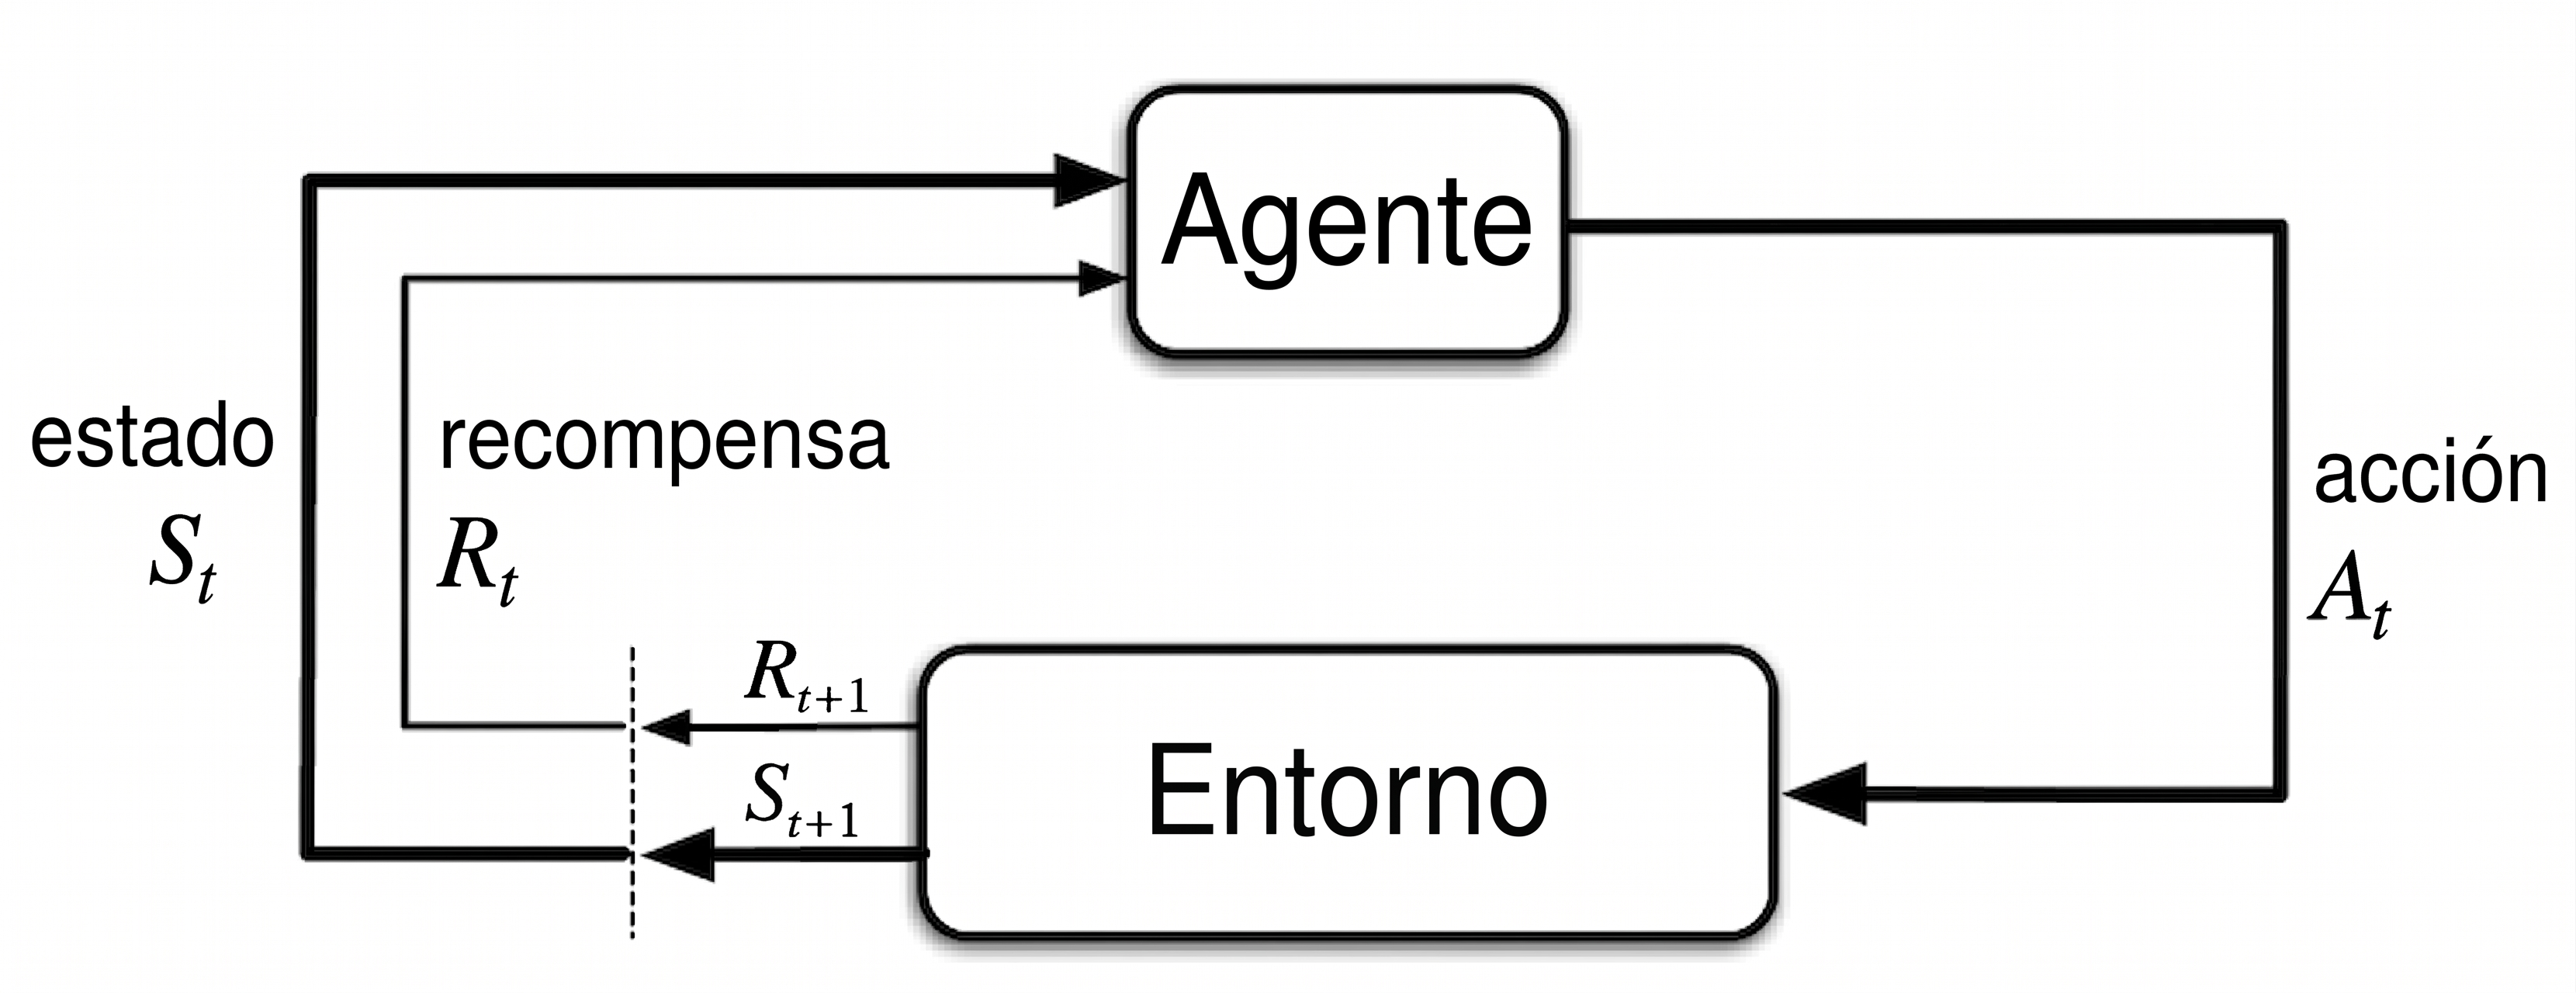
\includegraphics[width=0.6\textwidth]{imaxes/03_marco/rl_basics.png}
    \caption[Ilustración del proceso básico de aprendizaje por refuerzo]{Proceso iterativo del aprendizaje por refuerzo.
    El agente observa el estado del entorno, ejecuta una acción según su \gls{política} y recibe una recompensa y un nuevo estado. 
    Adaptada de \textit{Reinforcement Learning: An Introduction}~\cite{DBLP:books/lib/SuttonB2018}.}
    \label{fig:rl-basics}
\end{figure}

El problema se plantea habitualmente como un \gls{mdp}~\cite{DBLP:books/wi/Puterman94}, que formaliza la interacción 
asumiendo que el siguiente estado y la recompensa dependen únicamente del estado actual y la acción tomada:
\begin{equation}
    P(X_{n+1} = j \mid X_n = i, A_n = a)
\end{equation}
donde $X_n$ es el estado en el instante $n$ (con valor $i$), $A_n$ la acción tomada en ese
instante ($a$) y $X_{n+1}$ el estado resultante (con valor $j$); es decir, la probabilidad
de transitar al estado $j$ depende únicamente del estado y la acción actuales.
    
El objetivo del agente, por tanto, es maximizar el \textit{retorno esperado}, definido como la suma
descontada de las recompensas obtenidas a lo largo de la interacción:
\begin{equation}
    J(\pi) = \mathbb{E}_{\pi}\!\left[\sum_{t=0}^{\infty} \gamma^{t}\, r_t\right]
\end{equation}
donde $r_t$ es la recompensa recibida en el paso $t$, $\gamma \in [0,1)$ es el
\textit{factor de descuento} (que resta peso a las recompensas más lejanas) y
$\mathbb{E}_{\pi}[\cdot]$ denota el valor esperado siguiendo la \gls{política} $\pi$.

Para evaluar la calidad de las decisiones se define la \textit{función de valor-acción}
$Q^{\pi}(s,a)$, que estima el retorno esperado al ejecutar la acción $a$ en el estado $s$
y seguir después la \gls{política} $\pi$:
\begin{equation}
    Q^{\pi}(s,a) = \mathbb{E}_{\pi}\!\left[\sum_{t=0}^{\infty} \gamma^{t}\, r_t
    \;\middle|\; s_0 = s,\; a_0 = a\right]
\end{equation}

Esta función satisface la \textit{ecuación de Bellman}, que divide un problema complejo en subproblemas más simples, expresando el valor de una decisión actual en función de la recompensa inmediata y del valor de los estados futuros. Con ello, se puede expresar de forma recursiva
en términos del estado y la acción siguientes ($s'$ y $a'$):
\begin{equation}
    Q^{\pi}(s,a) = \mathbb{E}\!\left[\, r + \gamma\, \mathbb{E}_{a'\sim\pi}\big[Q^{\pi}(s',a')\big]\,\right]
\end{equation}

Aunque la ecuación de Bellman propaga teóricamente el valor hacia las decisiones anteriores,
en tareas de largo horizonte con recompensas escasas esta propagación se vuelve lenta y la señal
de aprendizaje se debilita: el agente apenas recibe recompensa hasta completar una secuencia larga
de acciones, lo que dificulta en la práctica atribuir correctamente el valor a cada decisión.
Para mitigar esto se utilizan recompensas intermedias (\gls{reward-shaping}) que guían la exploración.

Por ejemplo, en la tarea de \gls{woodcutting}, si solo se premiara talar árboles, el agente no aprendería cómo orientarse, 
moverse o interactuar con el entorno. Por ello se añaden recompensas intermedias por aproximarse al árbol, apuntar o golpearlo.

En este trabajo se analizan tres familias de \gls{drl}, diferenciadas de los enfoques clásicos por el uso de 
\gls{aprendizaje-automatico} para aprender la \gls{política}:

\begin{itemize}
    \item \textbf{Basados en valor}: aprenden una función $Q(s,a)$ y seleccionan la acción de mayor valor. 
    El ejemplo más representativo son las \gls{dqn}~\cite{DBLP:journals/nature/MnihKSRVBGRFOPB15}, 
    que usan redes neuronales y un \gls{replay-buffer}.

    \item \textbf{Gradiente de \gls{política}}: optimizan directamente la \gls{política} mediante ascenso de gradiente. 
    El referente es \gls{ppo}~\cite{DBLP:journals/corr/SchulmanWDRK17}.

    \item \textbf{Actor-crítico}: combinan ambos enfoques, con un actor que produce la \gls{política} y 
    un crítico que evalúa su calidad. El referente es \gls{sac}~\cite{DBLP:journals/corr/abs-1801-01290}.
\end{itemize}

Se añade una taxonomía adicional~\cite{DBLP:books/lib/SuttonB2018}, ilustrada en la Figura~\ref{fig:on-vs-off} (página~\pageref{fig:on-vs-off}):

\begin{itemize}
    \item \textbf{\Gls{on-policy}}: el agente aprende de la \gls{política} que ejecuta.
    \item \textbf{\Gls{off-policy}}: el agente aprende de experiencias generadas por \glspl{política} anteriores mediante un \gls{replay-buffer}.
\end{itemize}

% No les pongo aqui el resize pa que entren bien
\begin{figure}[htbp]
    \centering
    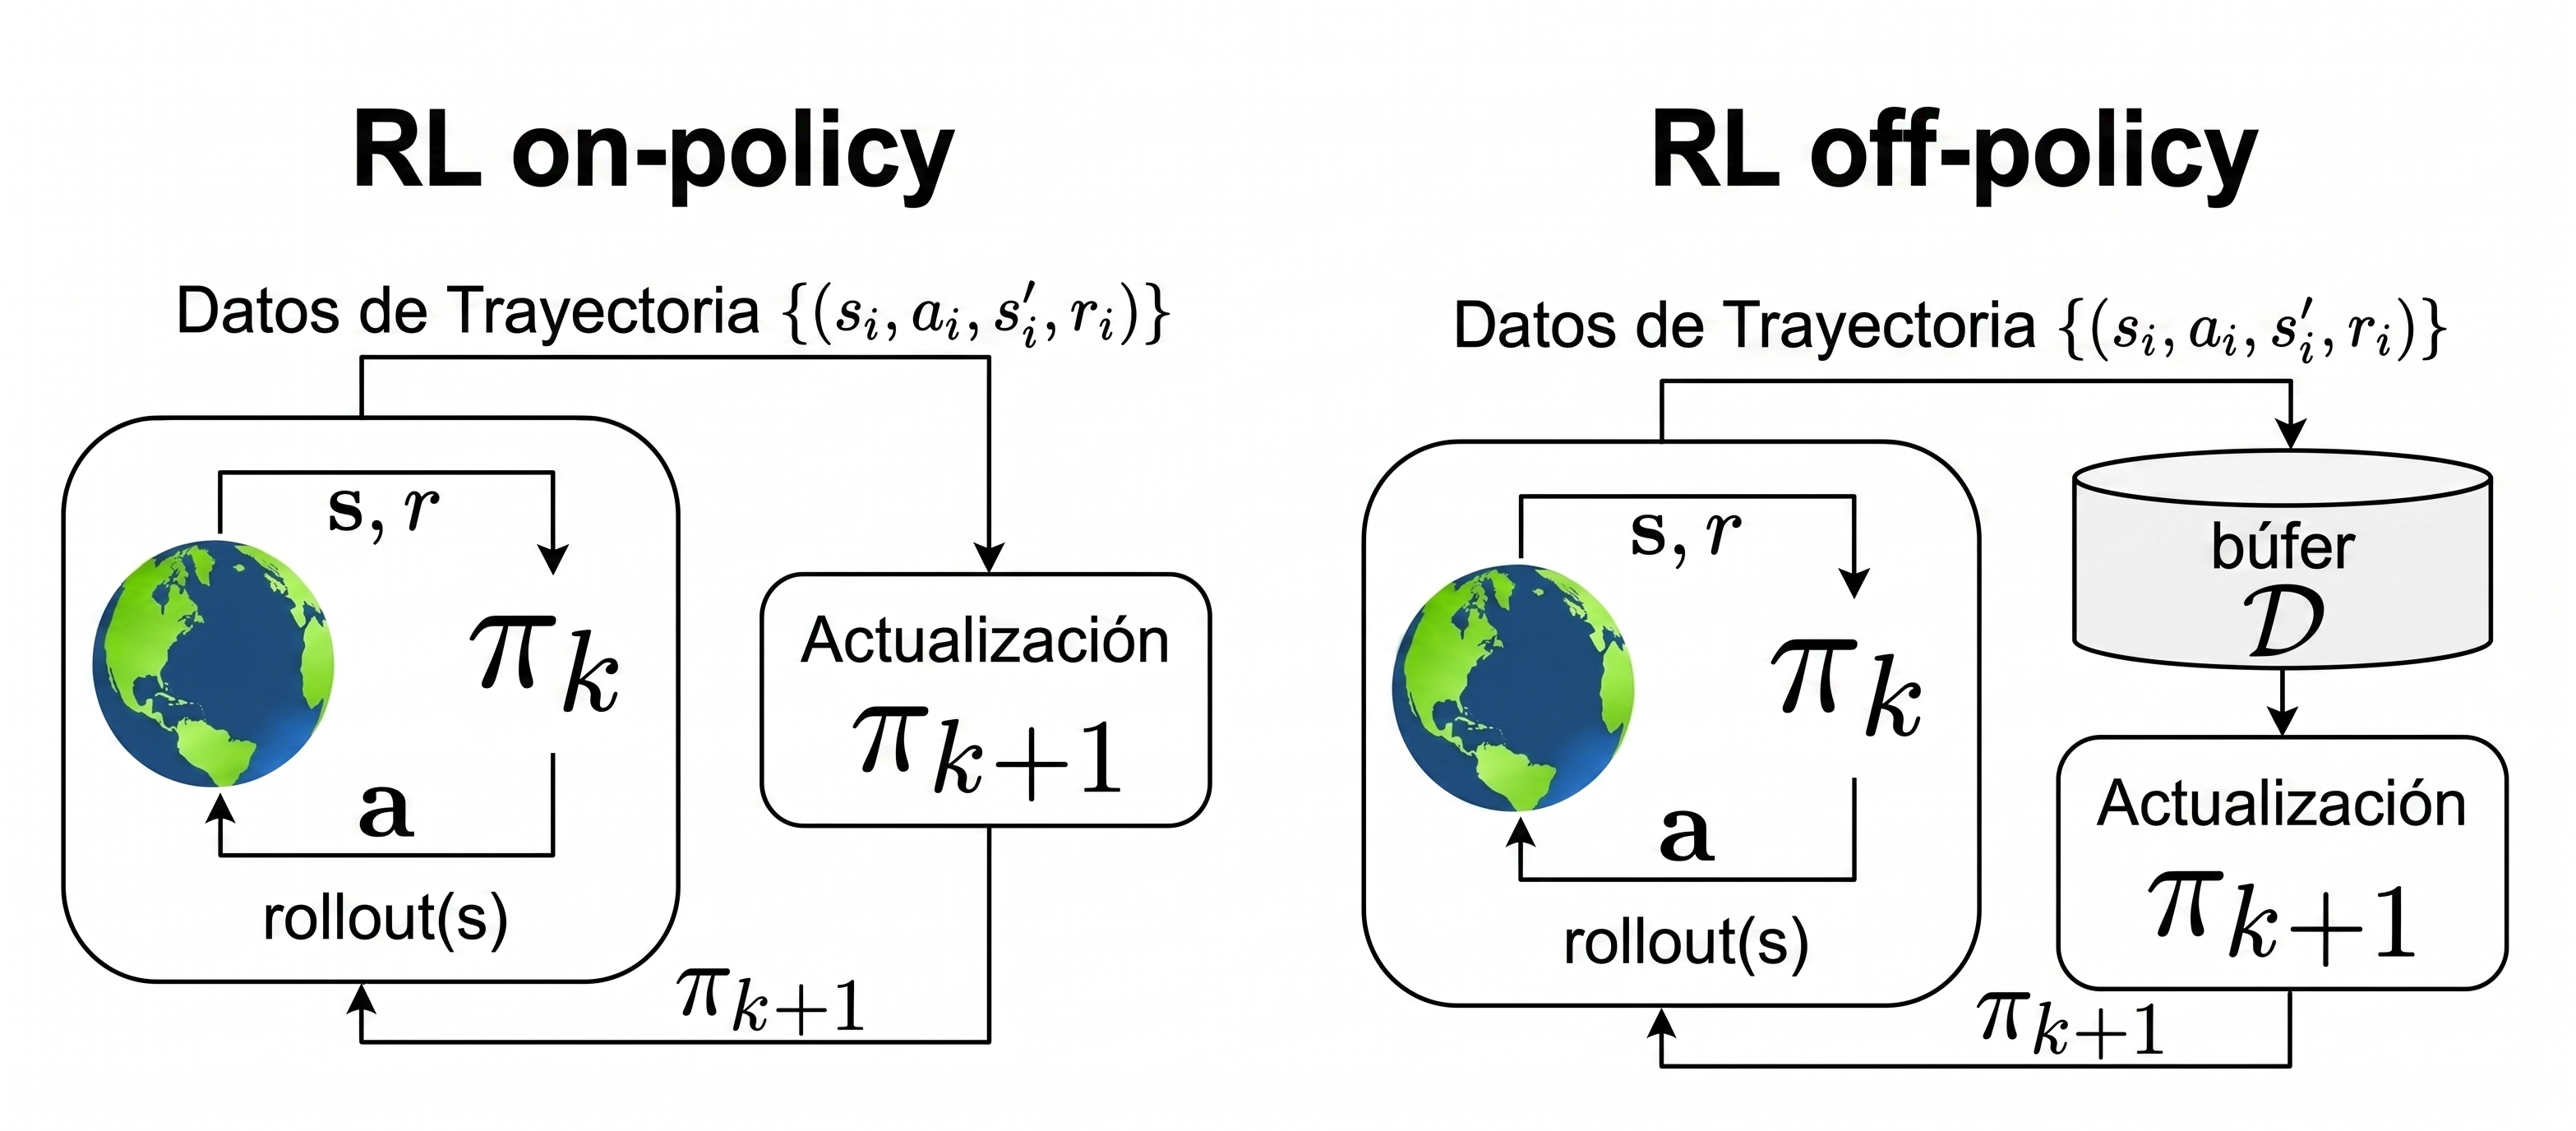
\includegraphics[width=0.55\textwidth]{imaxes/03_marco/on_vs_off.png}
    \caption[On-policy vs off-policy]{Diferencia entre enfoques \gls{on-policy} y \gls{off-policy}. 
    Adaptada de \textit{Offline Reinforcement Learning: Tutorial, Review, and Perspectives on Open Problems}~\cite{DBLP:journals/corr/abs-2005-01643}.}
    \label{fig:on-vs-off}
\end{figure}